% ------------------------------------------------------------------------
% PROPRIEDADES DO DOCUMENTO
% ------------------------------------------------------------------------
\documentclass[12pt,
openright, 
oneside, %
%twoside, %TCC: Se seu texto tem mais de 100 páginas, descomente esta linha e comente a anterior
a4paper,    %
%english,   %
brazil]{facom-ufu-abntex2}

% ------------------------------------------------------------------------
% PACOTES
% ------------------------------------------------------------------------
\pdfstringdefDisableCommands{\let\uppercase\relax}
\usepackage{amsmath}
\usepackage{icomma}
\usepackage[portuguese,ruled]{algorithm2e}
\usepackage{float}
\usepackage{multirow}

% ------------------------------------------------------------------------
% INFO para CAPA e FOLHA DE ROSTO 
% ------------------------------------------------------------------------
\titulo{Análise de conteúdo sobre vulnerabilidades de segurança em redes sociais} %TCC

\autor{Rodrigo Borges Machado} %TCC
\data{2019}

\orientador{Rodrigo Sanches Miani} %TCC
%\coorientador{Nome completo do orientador caso tenha} %TCC

\begin{document}
\frenchspacing 

% ----------------------------------------------------------
% ELEMENTOS PRÉ-TEXTUAIS
% ----------------------------------------------------------
%\pretextual
\imprimircapa
\imprimirfolhaderosto


% --- Inserir folha de aprovação --- %
\begin{folhadeaprovacao}

  \begin{center}
    {\ABNTEXchapterfont\large\imprimirautor}

    \vspace*{\fill}\vspace*{\fill}
    {\ABNTEXchapterfont\bfseries\Large\imprimirtitulo}
    \vspace*{\fill}
    
    \hspace{.45\textwidth}
    \begin{minipage}{.5\textwidth}
        \imprimirpreambulo
    \end{minipage}%
    \vspace*{\fill}
   \end{center}
    
   Trabalho aprovado. \imprimirlocal, 20 de dezembro de 2018: %TCC:

   \assinatura{\textbf{\imprimirorientador} \\ Orientador}  
   \assinatura{\textbf{Maria Adriana Vidigal de Lima} \\Professora}% \\ Convidado 1} %TCC:
   \assinatura{\textbf{Renan Gonçalves Cattelan} \\Professor}% \\ Convidado 2} %TCC:
   %\assinatura{\textbf{Professor} \\ Convidado 3}
   %\assinatura{\textbf{Professor} \\ Convidado 4}
      
   \begin{center}
    \vspace*{0.5cm}
    {\large\imprimirlocal}
    \par
    {\large\imprimirdata}
    \vspace*{1cm}
  \end{center}
  
\end{folhadeaprovacao}
% \includepdf{folhadeaprovacao_final.pdf} % TCC: depois de aprovado o trabalho, descomente esta linha e comente a anterior para incluir o scan da folha de aprovação.

%% OBS.: as seções dedicatória, agradecimento e epígrafe não são obrigatórias. Só as mantenha se achar pertinente.

% --- Dedicatória --- %
\imprimirdedicatoria{Aos meus pais
Hélio Antônio Machado e
Maria Alice Borges da Silveira e \\irmãs Andréa Caroline Machado, Andressa Borges Machado, Luciana Cristina Machado e Simone Cristina Machado}

% --- Agradecimentos --- %
\imprimiragradecimentos{
Agradeço primeiramente a Deus, por possibilitar que eu caminhasse por todo esse caminho de luta com a cabeça sempre erguida, com força para passar pelos obstáculos e saúde para seguir lutando.

Aos meus pais por todo amor, carinho, incentivo e apoio que sempre me deram. Por sempre me incentivarem a buscar mais, a querer mais, e nunca parar de lutar. Por possibilitar uma educação boa e ensinar a ter a humildade que a vida pede.

Às minhas irmãs por todo carinho, apoio e compreensão pelo tempo que tive que abdicar para dedicar a minha formação.

Aos meus amigos pelo incentivo e compreensão durante toda essa jornada. Principalmente por saberem como me animar quando estava em momentos difíceis. Obrigado à Confraria por existir e me fazer tão bem.

À minha namorada Milena Bertolini que sempre esteve ao meu lado enquanto fiz esse trabalho. Obrigado pelo carinho e por todo amor que me deu. Desculpe pelos compromissos cancelados, teremos toda a vida para compensar. Obrigado por estar sempre ao meu lado.

A todos os professores que me insentivaram, desde os professores do meu ensino fundamental, médio e agora no ensino superior. Um obrigado especial aos professores do Instituto Federal do Triângulo Mineiro, que sempre me ajudaram mesmo depois de eu já ter formado no ensino médio.

Ao meu orientador, Professor Doutor Rodrigo Miani, pela paciência, prontidão e confiança. Obrigado por ser sempre um amigo desde as aulas na classe, até no stress desse trabalho. Obrigado por ter sempre um tempo para poder conversar, seja assunto pessoal ou não.
}

% --- Epígrafe --- %
\imprimirepigrafe{"Que todos os nossos esforços estejam sempre focados no desafio à impossibilidade. Todas as grandes conquistas humanas vieram daquilo que parecia impossível."\\Charles Chaplin.}
	
% --- Resumo em português --- %
%
\begin{resumo} %TCC:
Esse trabalho utiliza conceitos de análise de dados para avaliar a ocorrência de vulnerabilidades descobertas em sistemas operacionais Windows, sistemas operacionais diferentes do Windows e aplicações Web nos últimos dez anos usando uma base de dados pública mantida pelo NIST \textit{(National Institute of Standards and Technology)}. Ao longo da pesquisa foi utilizado o cálculo de índice de sazonalidade e a função de autocorrelação para investigar se as tendências encontradas em um estudo anterior continuam as mesmas, além de analisar vulnerabilidades presentes em softwares que não foram contemplados em tal trabalho. Os resultados encontrados indicam duas tendências de sazonalidade: aumento de vulnerabilidades reportadas em junho para todos os sistemas operacionais investigados e diminuição do número de vulnerabilidades em janeiro em todos os softwares analisados.


%% Rodrigo - complemente com uma frase sobre os resultados. Algo do tipo: "Os resultados mostram que..."
 
  \vspace{\onelineskip}
  \noindent
  \textbf{Palavras-chave}: Vulnerabilidade de Segurança, Segurança da Informação, CVE, Twitter, . %TCC:
 \end{resumo}

% --- lista de ilustrações --- %
\listailustracoes

% --- lista de tabelas --- %
\listatabelas

% --- lista de abreviaturas e siglas --- %
\begin{siglas} %TCC:
	
	% 0
	
	% 1
	
	% 2
	
	% 3
	
	% 4
	
	% 5
	
	% 6
	
	% 7
	
	% 8
	
	% 9
	
	% A
    \item[ACF] Análise da Função de Autocorrelação
    \item[AIC] Critério de Informação Akaike
    \item[AML] Modelo Logístico Alhazmi-Malaiya
    \item[AT] Modelo Termodinâmico
    \item[ARIMA] Modelo Auto-Regressivo Integrado de Médias Móveis
	
	% B
	
	% C
	\item[CSV] Comma Separated Values
    \item[CVE] Commom Vunerabilities and Exposures
	
	% D
	
	% E
	
	% F
	
	% G
	
	% H
    \item[HTTP] Hypertext Transfer Protocol
	
	% I
	\item[IE] Internet Explorer
    \item[IIS] Internet Information Services	
    
    % J
    \item[JSON] JavaScript Object Notation
	\item[JRE] Java Runtime Environment
    \item[JW] Modelo Weibull
	
	% K
	
	% L
    \item[LN] Modelo Linear
    \item[LP] Modelo Regressão de Poisson
	
	% M
    \item[SMB] Microsoft Server Message Block
	
	% N
    \item[NIST] National Institute of Standards and Technology
	\item[NVD] National Vulnerability Database
    
	% O
    \item[OS] Sistema Operacional
    \item[OSes] Sistemas Operacionais
    \item[OSVDB] Open Source Vulnerability Database
	
	% P
	
	% Q
	
	% R
    \item[RE] Modelo Exponencial
    \item[RGB] Modelo de Crescimento de Confiabilidade
    \item[RQ] Modelo Quadrático
	
	% S
	\item[SO] Sistema Operacional
    
	% T
    \item[TI] Tecnologia da Informação
	\item[TIC] Tecnologia da Informação e Comunicação
    
	% U
	
	% W
	\item[W3C] World Wide Web Consortium

	% V
    \item[VDM] Modelo de Descoberta de Vulnerabilidade
	
	% X
	\item[XML] Extensible Markup Language
	% Y
    \item[YF] Modelo Distribuição Normal Dobrada
	
	% Z
	\item[ZIP] Formato de extensão de um arquivo compactado

\end{siglas}




% --- lista de símbolos --- %
%\begin{simbolos}
	% 0
	
	% 1
	
	% 2
	
	% 3
	
	% 4
	
	% 5
	
	% 6
	
	% 7
	
	% 8
	
	% 9
	
	% A
	
	% B
	
	% C
	
	% D
	
	% E
	\item[$ \in $] Pertence
	
	% F
	\item[$F$] Valor falso do tipo de dado primitivo Booleano
	
	% G
	\item[$ \Gamma $] Letra grega Gama
	
	% H
	
	% I
	
	% J
	
	% K
	
	% L
	\item[$ \Lambda $] Lambda
	
	% M
	
	% N
	
	% O
	
	% P
	
	% Q
	
	% R
	
	% S
	
	% T
	
	% U
		
	% W
	
	% V
	\item[$V$] Valor verdadeiro do tipo de dado primitivo Booleano
	
	% X
	
	% Y
	
	% Z
	\item[$ \zeta $] Letra grega minúscula zeta
	
\end{simbolos} % caso não existe símbolos no trabalho, comente esta linha

% --- sumario --- %
\sumario


% ----------------------------------------------------------
% ELEMENTOS TEXTUAIS
% ----------------------------------------------------------
\textual

% --- Introdução --- %
% ----------------------------------------------------------
% Introdução
% ----------------------------------------------------------
\chapter[Introdução]{Introdução}

A rede de computadores do mundo se tornou de longe uma das principais evoluções da humanidade. A globalização é a prova de que todo o avanço funcionou e essa evolução foi necessária. Nesse contexto, a pesquisa sobre segurança da informação foi ampliada, principalmente devido à necessidade.

As vulnerabilidades de sistema entram em contraste com esse acelerado crescimento. Elas mostram como sistemas de grandes empresas podem, facilmente, perecer sob ataques. Os atacantes em sua essência mostram seus poderes no momento do pós ataque, principalmente em redes sociais, quando postam o que fazem, muitas vezes disponibilizando instruções de como fazer.

No contexto da segurança de computadores, vulnerabilidades são falhas ou fraquezas de softwares que permitem a agentes maliciosos subverterem o uso originalmente desejado de algum sistema computacional e violarem políticas de segurança \cite{Belarmino2014}. 

O número de vulnerabilidades que são encontradas em sistemas, nos últimos anos, cresceu de forma exponencial. Isso não significa que todas descobertas foram exploradas. A grande quantidade de demanda para uma baixa quantidade de produção de reparos faz com que apenas vulnerabilidades julgadas como críticas sejam exploradas, uma vez que as restantes são deixadas de lado.

Sistemas inteiros podem ser tomados por hackers, que conseguem ter informações sigilosas sobre os usuários de um serviço, ou mesmo da empresa que mantém tal sistema. Além disso, hackers muitas vezes estorquem empresas a pagarem elevadas quantias para terem seus sistemas e dados privados de volta. 

A discussão sobre as vulnerabilidades em redes sociais mostram como o assunto é tomado pelo público. Assim, pessoas passam a entender mais sobre sistemas e seus bugs, começam a identificar quais são as formas de se identificar vulnerabilidades e quais os passos para apresenta-las ao mundo para que sejam exploradas de maneira legal.

O número de pessoas que discutem temas como vulnerabilidades e bugs em sistemas têm crescido exponencialmente nos últimos anos. O foco é conseguir reduzir o número de falhas em sistemas.

O objetivo desse trabalho é identificar as vulnerabilidades que são discutidas na rede social do twitter, tais como seus aspectos e a possibilidade de ser exploradas. O foco é analisar o volume de dados de discussão sobre esse tópico na rede social, a fim de entender se há um aumento na atenção desse assunto.

Com o crescimento ascendente de novas tecnologias que proporcionam novos sistemas, os backdoors são explorados cada vez mais. A busca pelas vulnerabilidades estão nesse meio para listar quais os possíveis problemas nelas e o que pode ser feito para contorna-las.

Afim de listar as vulnerabilidades discutidas e o volume dessas informações, será criado um sistema que vasculhe o Twitter por publicações sobre o assunto limitando entre uma data x e y. Assim, será possível, através de mineração de dados, quais são as vulnerabilidades mais discutidas, quais os usuários que normalmente fazem tais publicações e o quão retwitadas elas são.

% ------------------%
% --- Objetivos --- %
%\section{Objetivos}


% -------------------%
% --- Resultados --- %
%\section{Resultados esperados}

%\section{Organização do Trabalho}


% ---  Fundamentação teórica --- %
% ----------------------------------------------------------
% revisão bibliográfica
% ----------------------------------------------------------
\chapter[Revisão Bibliográfica]{Revisão Bibliográfica}

Este capítulo apresenta um levantamento bibliográfico sobre segurança da informação e vulnerabilidades. Tem como objetivo definir conceitos e apresentar exemplos da utilização dos termos e seus exemplos no mundo real. Será listada as definições e as ténicas utilizadas para efetuar o trabalho e como serão considerados os dados para sua utilização posterior. Será considerado ainda as ferramentas a ser utilizadas para a busca da pesquisa.

% --------------------------%
% --- Conceitos Básicos --- %
\section{Segurança da Informação}

Segurança da Informação é o conjunto de orientações, normas, procedimentos, políticas e demais ações que têm por objetivo proteger o recurso informação, possibilitando que o negócio da organização seja realizado e a sua missão seja alcançada \cite{Fontes2017}. Assim, a segurança é o pilar principal de pesquisa desse trabalho.  Quando se envolve segurança de sistemas, de redes, de serviços etc; se resume tudo em segurança da informação.  

Proteger a informação é responsabilidade de cada usuário na organização em que coopera e cabe à organização orientar seus colaboradores em relação à proteção da informação. De acordo com \citeonline{Spanceski2004}, uma das formas de proteger a informação é conhecer os pilares da área da segurança da informação. Esses, são considerados as divisões dessa ciência que juntos formam toda a segurança da informação. São:

\begin{itemize}
\item Integridade: pilar que assegura que sistemas e informações serão modificados apenas nas condições previstas, assim impede que sejam manipuladas afetando os usuários. A integridade é a garantia da exatidão e completeza da informação e dos métodos de processamento \cite{ABNT2005};
\item Disponibilidade: garante que os dados, sistemas e serviços estejam disponíveis para aqueles que tem o direito de utilizá-los. A disponibilidade é a garantia de que os usuários autorizados obtenham acesso à informação e aos ativos correspondentes sempre que necessário \cite{ABNT2005}.
\item Confidencialidade: esse pilar assegura que as informações não serão acessadas por agentes não autorizados. A confidencialidade é a garantia de que a informação é acessível somente por pessoas autorizadas a terem acesso \cite{ABNT2005}.
\end{itemize}

A integridade de uma mensagem A é o conceito de que não há nenhuma alteração em seu conteúdo mantendo sua estrutura original. Garantir sua integridade significa não permitir que a informação seja modificada, alterada ou mesmo destruída, que seja legítima e permancessa consistente \cite{Dantas2011}.

Ocorre a não integridade de uma informação quando seu conteúdo é corrompido, falsificado, roubado ou destruído \cite{Dantas2011}. Quando uma informação está íntegra, então seus dados são seguros e há a garantia que são originais.

A disponibilidade reporta a garantia de que uma informação está acessível. Deste modo, não se restringe apenas a algum sistema online estar apto a se conectar, mas uma informação que esteja ao alcance dos usuários destinatários.

Quando não há disponibilidade significa que a informação não está disponível para ser utilizada, ou seja, está fora do alcance dos usuários destinatários \cite{Dantas2011}. 

Para ter disponibilidade deve ser assegurando a garantia da leitura e acesso da informação no momento em que se necessita da mesma.

A confidencialidade é a certeza de que uma informação é acessível apenas para o remetente e para o destinatário, sendo que qualquer outro terceiro não consiga ter a informação encaminhada. A garantia da confidencialidade é deixar de que outro terceiro não tenha acesso à informação original e que não possa divulga-la. 

É natural que com a evolução e o desenvolvimento a segurança da informação tenha se focado muito na área de comunicação de dados e informação. Esse fato, abre porta para outras pontas de atenção, como:

\begin{itemize}
\item Autenticidade: garante que a mensagem é do próprio remetente. É a garantia de que a informação é oriunda da fonte que lhe é atribuída e elaborada por quem tem autoridade para tal. Diz respeito à idoneidade da fonte, ou seja, digna de confiança \cite{Dantas2011};
\item Confiabilidade: garante que a fonte emitente da mensagem é confiável e autêntica. É a garantia de que a informação é confiável, oriunda de uma fonte autêntica e que expressa uma mensagem verdadeira. Diz respeito ao conteúdo \cite{Dantas2011}.
\item Não repúdio: garante que a informação sempre chegará ao destino final e será sempre interpretada. É a garantida de que a informação chegará ao destino certo e não será repudiada. \cite{Dantas2011}.
\item Responsabilidade: é o agregado de responsabilidade de todos os envolvidos na criação, armazenamento e transporte da informação. É a coparticipação de responsabilidades por todos os que produzem, manuseiam, transportam e descartam a informação, seus sistemas e redes de trabalho. \cite{Dantas2011}.
\end{itemize}

Com esse conjuto de propriedades presente na comunicação em rede \cite{ABNT2005}, o remetente tem a garantia de quem recebe suas informações é realmente o destinatário que se diz ser. Garante ainda que a informação recebida está exatamente igual à enviada pelo remetente. Assegura também que nem o emissor nem o remetente neguem que houve comunicação.

\section{Vulnerabilidades de Segurança}
A quebra da segurança da informação indica que um sistema ou serviço foi violado, ou seja, algo em sua essência possibilitou que algum atacante conseguice penetrar em suas camadas a ponto de encontrar uma forma de roubar uma informação, por exemplo. Isso é considerado uma vulnerabilidade do sistema. 

No contexto de segurança da informação, vulnerabilidade pode ser uma falha em um sistema ou serviço que permita realização e concretização de um ataque \cite{Aparecido2014}. Para que um atacante consiga explorar essa vulnerabilidade, ele precisa de um meio ou ferramentas que possibilite seu ataque, assim ele conecta com a fraqueza do sistema ou serviço, essas ferramentas ou mesmo tecnicas são chamadas de exploits \cite{Whitman2011}.

A figura \ref{fig:xiao} representa o ciclo de vida de uma vulnerabilidade. De modo geral, uma vulnerabilidade tem o seu descobrimento e, a partir disso, há os passos para soluciona-lo. Representando um sistema que esteja já em base de produção, a vulnerabilidade se destaca como um bug, mas não um simples bug, mas sim um que tenha postencial de afetar o sistema. No modo de produção do sistema, a equipe então desenvolverá uma versão que corrija aquele bug e liberará essa correção, seja como um instalador de sistema, para aplicativos desktop ou mesmo para mobile, ou então irá subir no servido, caso seja um site ou serviço de API. 

\begin{figure}[H]
\centering
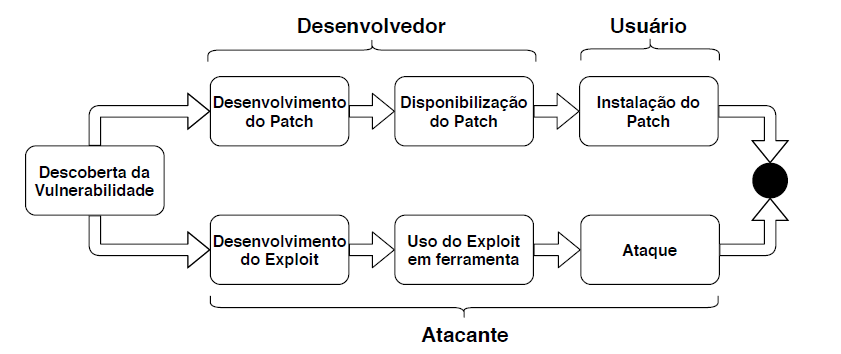
\includegraphics[width=1\textwidth]{imagens/figura_xiao.PNG}
\caption{Ciclo de vida de uma vulnerabilidade \cite{xiao2018patching}}
\label{fig:xiao}
\end{figure}

O ciclo de vida de um software é vinculado com essa parte de desecoberta de vulnerabilidades, muita das vezes é até previsto no projeto. Quando se encontra algum bug ou backdoor que leve a algum ponto crítico de atenção, a equipe de desenvolvimento do sistema, serviço ou software, tem a responsabilidade de disponibilizar uma nova versão tal que a correção seja disponibilizada.

Existe ainda as ameaças que o software pode enfrentar, dessas são descobratas as vulnerabilidades. A saber \cite{Pfleeger2015}:

\begin{itemize}
\item Falhas no software ou no Hardware. Desde parâmetros externos, como fator ambiental, a fator interno como falta de memória.
\item Erros de usabilidade ou falha de administração.
\item Erros no projeto e de implementação.
\end{itemize}

Em sumo, não é possível a construção de uma lista que contenha todas as possíveis ameaças existentes. As formas de se encontrar vulnerabilidades em sistemas é diferente em cada tentativa e identificação de vulnerabilidade \cite{Pfleeger2015}. Como exemplo, o livro \citeonline{Pfleeger2015} apresenta a figura \ref{fig:vulnerabilidadeAgua} que faz uma analogia de uma vulnerabilidade do sistema.

\begin{figure}[H]
\centering
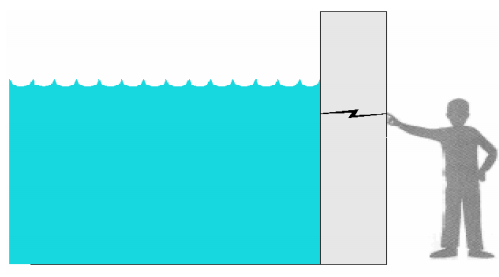
\includegraphics[width=1\textwidth]{imagens/vulnerabilidadeAgua.png}
\caption{Ameaça e Vulnerabilidade \cite{Pfleeger2015}}
\label{fig:vulnerabilidadeAgua}
\end{figure}

Depois de lançado um software inicia a fase de descoberta de vulnerabilidades. Essa fase não é composta apenas pela equipe de desenvolvimento do sistema/serviço, mas também dos usuários. Atacantes entram nesse contexto até mesmo como aliados para descoberta de aberturas, o problema existe quando eles tentam tirar proveito disso. Quando descoberto vulnerabilidades, essas podem ser divulgadas ao público através de fóruns públicos ou mesmo quando liberado correção de tal vulnerabilidade.

Redes sociais são um caminho também de divulgação de problemas em sistemas e serviços. O twitter, base desse trabalho, tem um número de dados muito grande referente à discussão de problemas como esse, que será apresentado posteriormente.

Vários órgãos e departamentos ligados a segurança da informação como o NIST (National Institute of Standards and Technology), FIRST (Forum of Incident Response and Security Teams), CERT (Computer Emergency Response Team) entre outros, se juntaram para criar um padrão para pontuação/mensuração de vulnerabilidades de software chamado de CVSS [Schiffman (2005)] \cite{Peotta2006}. 

Alguns dos dados sobre vulnerabilidades e falhas de segurança são apresentados ao público através de sites específicos a esse fim. Esses sites armazenam informações sobre tais incidentes e possibilitam buscas em cima deles. Sites como as organizações NVD \cite{NVD}, Secunia \cite{Secunia2009}, US-CERT \cite{CERT1991} e \textit{Open Source Vulnerability Database} \cite{OSVDB2002}.

O NVD é uma referência na coleta de dados sobre vulnerabilidade e é sincronizado com o CVE \textit{(Common Vulnerabilities and Exposures)} \cite{CVE1985}. Enquanto o CVE cadastra vulnerabilidades, o NVD categoriza e avalia os riscos delas. Ademais, o CVE apresenta de modo simples detalhes sobre a vulnerabilidade, exploits e se há correção. Ele é um banco de dados público, logo qualquer usuário tem acesso à sua base de conhecimento. O principal gestor do portal é o MITRE \textit{(Massachusetts Institute of Technology's Digital Computer Laboratory)}, que além de disponibilizar a informação tem a intenção de padronizar esses dados com a ajuda do NVD \cite{Peotta2006}. 

Pelo site do NVD, asism como no CVE, é possível listar as vulnerabilidades. No site do CVE a organização dessa informação não tem uma boa visualização, enquanto no NVD é listado de forma fácil e interpretável. O site do CVE fornece possibilidade de baixar um arquivo contendo as vulnerabilidades filtrando por ano e possibilitando vários tipos de arquivos diferentes, como apresentado na Figura \ref{fig:cve1}.

\begin{figure}[H]
\centering
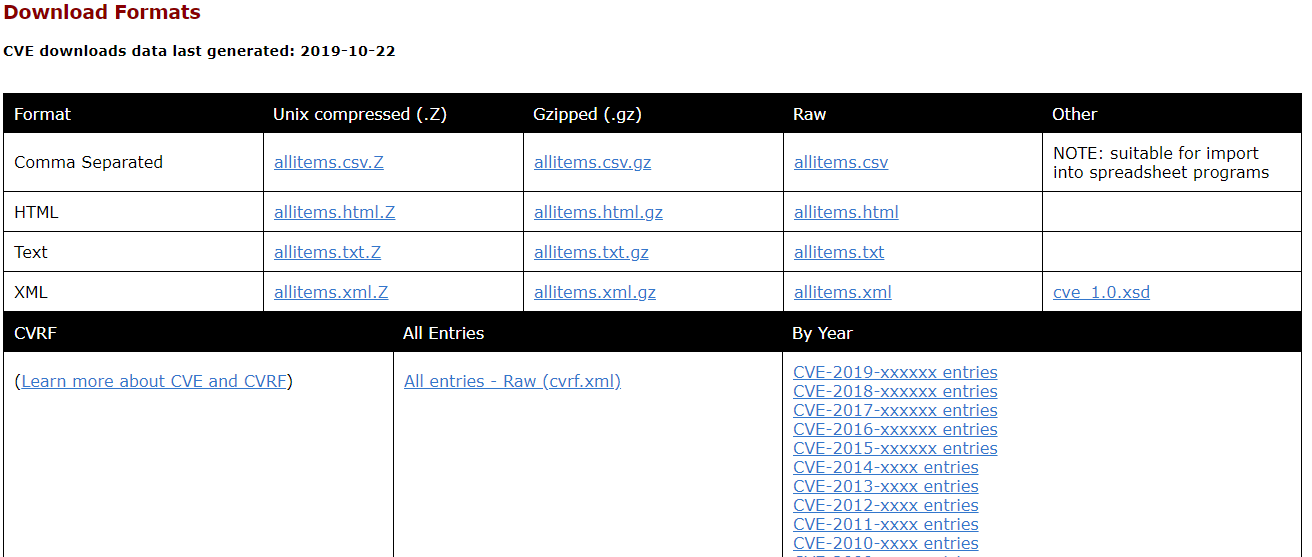
\includegraphics[width=1\textwidth]{imagens/cve_exemplo1.png}
\caption{Lista de opções de donwload de arquivos contendo vulnerabilidades}
\label{fig:cve1}
\end{figure}

Esses arquivos para download contém as vulnerabilidades do período selecionado. Caso selecionado o tipo, na primeira linha da tabela, é baixado todo um arquivo com aquela extensão selecionada e no formato desejado. Nesse arquivo será colocado todas as vulnerabilidades desde 1999. Quando baixado uma lista de vulnerabilidades de algum ano em específico, é carregado uma página web em xml com os dados daquele ano. A imagem \ref{fig:cve1_detalhes} mostra a configuração de um arquivo xml de exemplo.

\begin{figure}[H]
\centering
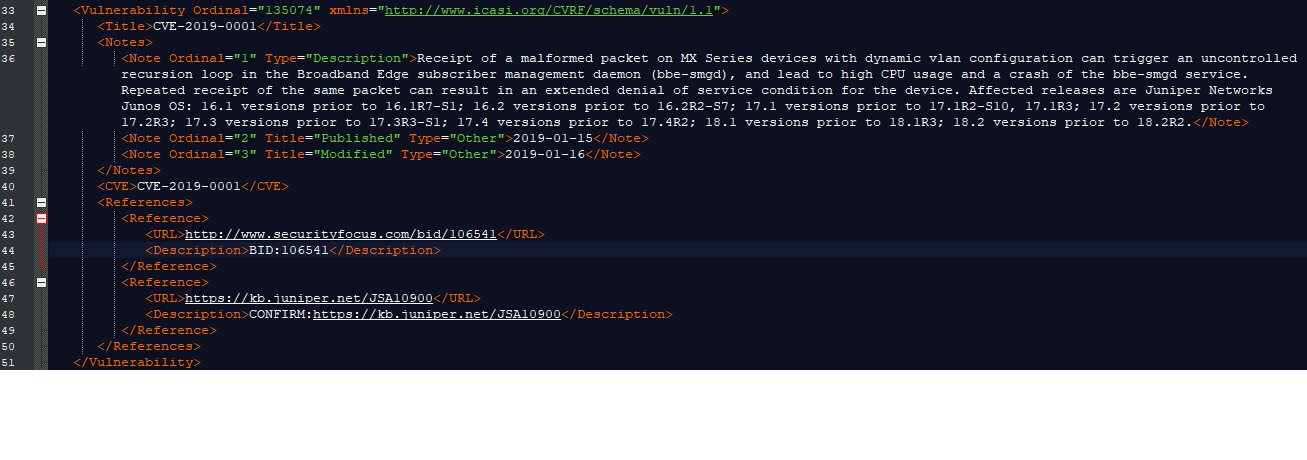
\includegraphics[width=1\textwidth]{imagens/cve1_detalhes.png}
\caption{Arquivo xml exemplificando uma vulnerabilidade de janeiro de 2019}
\label{fig:cve1_detalhes}
\end{figure}

Desse modo, o arquivo xml a ser baixado com as vulnerabilidades possibilita uma busca por códigos e até mesmo textos nas ocorrências, o que será utilizado no trabalho a fim de buscar os resultados com as postagens no twitter.

O site da NVD, entretanto, tem a possibilidade de listagem das vulnerabilidades através da seleção de um mês de algum ano, como apresentado na figura \ref{fig:nvd1}, filtrando o mês de setembro de 2019. Assim, é possível ter um filtro melhor caso esteja procurando apenas informações para uma leitura em específico.

\begin{figure}[H]
\centering
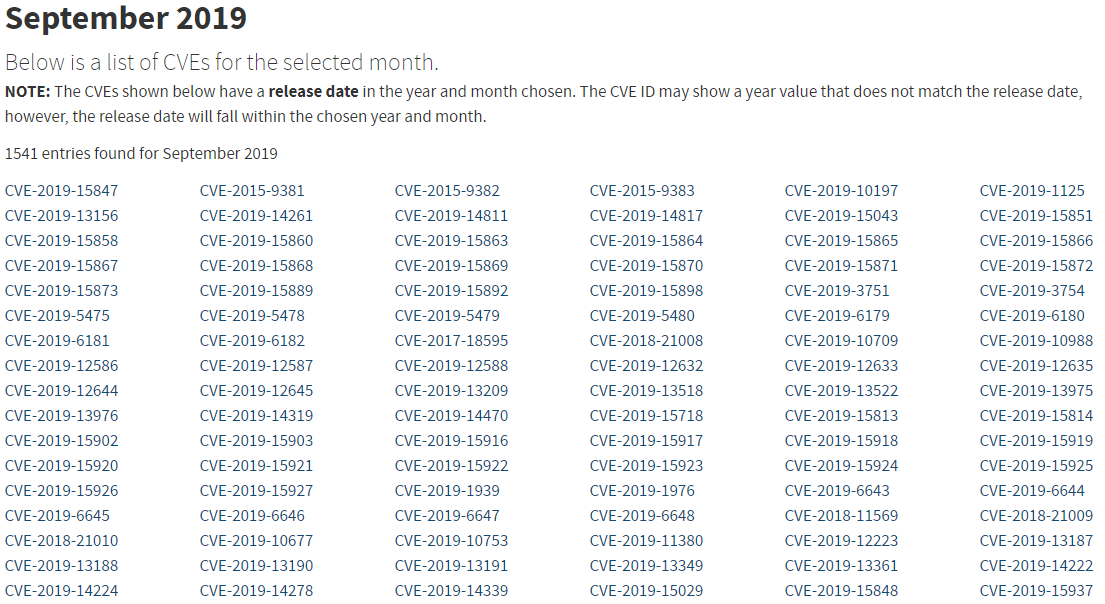
\includegraphics[width=1\textwidth]{imagens/nvd_exemplo1.png}
\caption{Vulnerabilidades reportadas pelo NVD em setembro de 2019}
\label{fig:nvd1}
\end{figure}

A Figura \ref{fig:nvd1} mostra parte das 1541 vulnerabilidades divulgadas para o mês de setembro de 2019. Quando selecionado algum CVE uma página é apresentando mostrando os detalhes daquela vulnerabilidade. Como um exemplo, o CVE-2019-15847 é apresentado na Figura \ref{fig:nvd3}.

\begin{figure}[H]
\centering
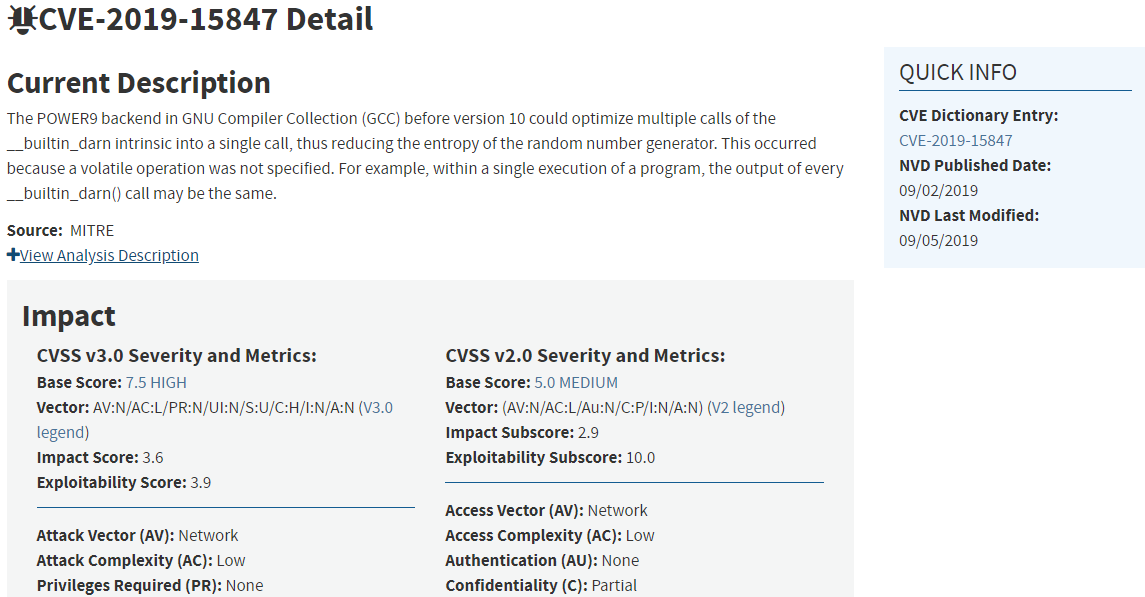
\includegraphics[width=1\textwidth]{imagens/nvd_exemplo3.png}
\caption{Vulnerabilidade CVE-2011-4042}
\label{fig:nvd3}
\end{figure}

A Figura \ref{fig:nvd3} apresenta os detalhes da vulnerabilidade CVE-2019-15847. Descrição \textit{(Description na Figura)}, a tabela de impacto \textit{(Impact na Figura)} e a data de publicação da vulnerabilidade \textit{(NVD Published Date na Figura)}, são alguns dos campos que são informados. Esses dados são oriundos do site da CVE e os mesmos arquivos xml que são possíveis de serem baixados são a base utilizada para a apresentação da informação. Logo, o site tem o proósito de apresentar a informação de uma forma mais legível e atraente para o usuário. 

O trabalho em questão utiliza esses dados do CVE como uma base de comparação de assuntos que estão postados no twitter. Dá-se então a estima para a listagem xml que possibilita uma mineração de dados em cima dos resultados obtidos do twitter.

% -------------------------------%
% --- Trabalhos Relacionados --- %
\section{Trabalhos Relacionados}

Esta seção tem o objetivo de descrever alguns trabalhos que têm relação ao tema principal desse projeto: discussão sobre vulnerabilidades em redes sociais. Os trabalhos \citeonline{Sabottke2015}, \citeonline{Correia2016}, \citeonline{ALVESBATISTA2007} e \citeonline{Kroth2018} serão apresentados posteriormente com o objetivo de descreve-los e vincula-los ao tema central desse trabalho. 

O número de vulnerabilidades tem crescido a cada ano, assim como é apresentado na figura \ref{fig:nvd1}, onde apenas no mês de setembro de 2019 é apresentado muitas novas incidências de bugs e backdoors. Esse crescimento é exponencial. Um outro exemplo que prova isso é que em 2014 foi o marco da primeira aparição de um CVE de 5 dígitos, pois o banco de dados do CVE [46], que atribui identificadores exclusivos às vulnerabilidades, adotou um novo formato que não limita mais o número de IDs do CVE a 10.000 por ano \cite{Sabottke2015}, assim é possível notar a quantidade crescente das vulnerabilidades, pois a nova métrica é incremental.

Um dos problemas é que esse crescimento de novas vulnerabilidades é muito maior que a capacidade de correções pela parte dos criadores \cite{ALVESBATISTA2007}. Nesse aspécto, tem-se a classificação qualitativa das vulnerabilidades encontradas. Essa classificação tem por objetivo identificar quais são as vulnerabilidades com  um nível de prioridade maior \cite{Sabottke2015}.

Com a ascensão do número de vulnerabilidades é necessário que haja aumento também do número de pessoas a combate-las. Nesse processo, o primeiro passo é identifica-las. As redes sociais estão nesse contexto, pois apresentam um meio que possibilita discussão sobre o assunto em questão. O Twitter, foco desse trabalho, é a rede social onde o assunto tem crescido, principalmente devido ao aumento de número de usuários, como apresentado na figura \ref{fig:relacionado_um}. em virtude das informações dos usuários obidas nessa rede social é possível, de forma automática, listar quais são as principais vulnerabilidades discutidas no momento e o quão importante elas são de serem sanadas e exploradas \cite{Correia2016}.

\begin{figure}[H]
\centering
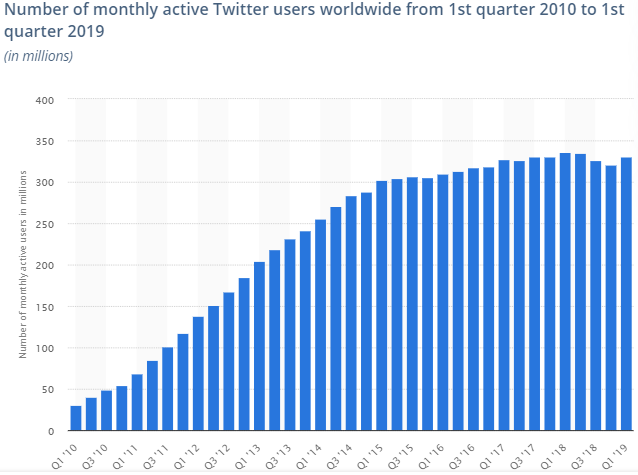
\includegraphics[width=1\textwidth]{imagens/relacionado_um.png}
\caption{Gráfico que apresenta o número de usuários na rede do Twitter entre os anos de 2010 e 2019 \cite{Statista2019}}
\label{fig:relacionado_um}
\end{figure}

\citeonline{Sabottke2015} é um trabalho que apresenta uma proposta de identificar, através de buscas no twitter, vulnerabilidades discutidas nessa rede social. Tem o objetivo de explorar qualitativa e quantitativamente os dados de vulnerabilidades disseminadas na rede \cite{Sabottke2015}. 

Muitas vulnerabilidades são encontradas e anunciadas diariamente. O capacidade de corrigir esses bugs é inversamente proporcional ao crescimento. \citeonline{Sabottke2015} então tenta propor uma forma de mensura das vulnerabilidades discutidas no Twitter, assim consegue levantar quais os problemas devem ser focadas primeiramente. Levanta também quais são os usuários que mantém essas discussões. Ademais, muitas das vulnerabilidades não têm grande impactos em sistemas, muitas vezes até sendo um falso-positivo, então o trabalho tem o objetivo de levantar apenas os bugs que realmente precisam ser corrigidos.

\citeonline{Sabottke2015} busca criar um sistema que filtre no tweets no Twitter através de alguma palavra chave e, a partir do resultado da busca, listar quais desses tweets falam sobre vulnerabilidades existentes e quais são exploráveis no mundo real. Para isso, o objetivo é criar um sistema que faça essa busca e essa sumarização qualitativa e quantitativa dos tweets, uma vez que essa tecnologia funcionará com a arquitetura apresentada na figura \ref{fig:Sabottke}.

\begin{figure}[H]
\centering
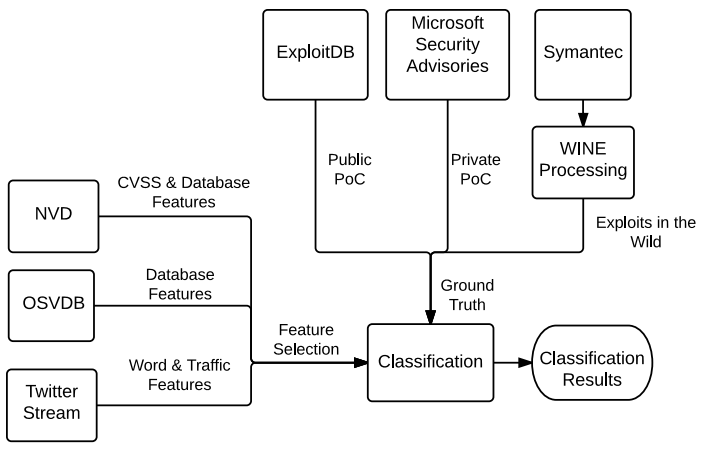
\includegraphics[width=1\textwidth]{imagens/Sabottke.png}
\caption{Arquitetura do sistema proposto pelo artigo \citeonline{Correia2016}}
\label{fig:Sabottke}
\end{figure}

Utilizando outras bases de segurança, o sistema se conecta à bases públicas como ExplitBD, Microsoft Security Advisories e Symantec, assim consegue filtrar as vulnerabilidades e buscar quais já foram exploradas. Essas bases de dados têm o objetivo de listar de forma organizada as vulnerabilidades com maior nível de atenção.

Assim, o sistema monta sua base de dados através do Twitter e faz a classificação, através das bases públicas de listagens de vulnerabilidades, de quais desses bugs devem ser tratados e fazendo o levantamento do quanto aparecem em publicações na rede social.

\citeonline{Correia2016} é um trabalho que utiliza de aprendizagem automática para conseguir identificar os tweets da rede social do Twitter que estão correlacionados à problemas de segurança de softwares e também relacionados à vulnerabilidades. Assim como \citeonline{Sabottke2015}, tem o objetivo de listar e filtrar de forma qualitativa e quantitativa as vulnerabilidades encontradas.

O autor tem como base o estudo de aprendizagem de máquina, uma vez que utiliza essa tecnologia com o objetivo de filtragem dos dados e, a partir dos resultados, melhorar a busca criando novos parâmetros para a pesquisa. O trabalho ainda lista uma série de restrições que a API utilizada para coleta dos dados tem, mas ainda sim apresenta seus resultados. A figura \ref{fig:Correia} apresenta a arquitetura utilizada para criação do sistema. Este é composto por duas fases, a representada a seguir é a fase de treino, onde é necessário o filtro humano para que o primeiro filtro seja feito. Essa necessidade se vê devido à natureza das técnicas de aprendizagem automáticas supervisionadas \cite{Correia2016}. Posterior a isso, o sistema consegue, através de aprendizagem, filtrar automaticamente os tweets de interesse. 

\begin{figure}[H]
\centering
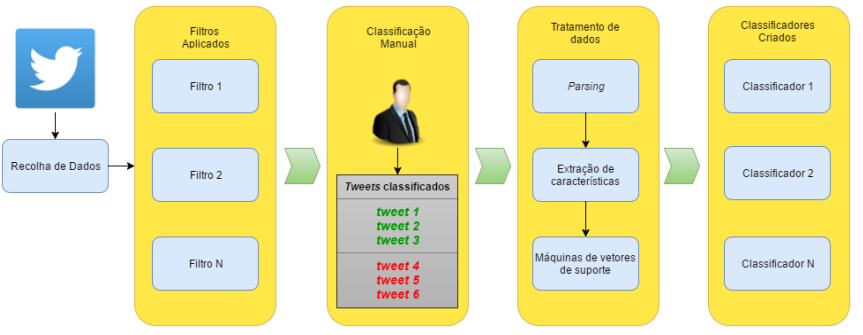
\includegraphics[width=1\textwidth]{imagens/Correia.png}
\caption{Arquitetura do sistema proposto pelo artigo \citeonline{Correia2016} representando a forma de treino do sistema}
\label{fig:Correia}
\end{figure}

Essa fase inicial tem o objetivo de, depois de recolidos os tweets, seja classificados por um analista quais são os dados relevantes em relação à ameaça de segurança à infraestrutura de TI. Após essa rotulação, o próprio sistema com os algoritmos de aprendizagem passa a conseguir um melhor resultado na obtenção de dados \cite{Correia2016}. Depois de treinado o sistema comporta de acordo com a arquitetura representada na figura \ref{fig:Correia2} no modo de operação.

\begin{figure}[H]
\centering
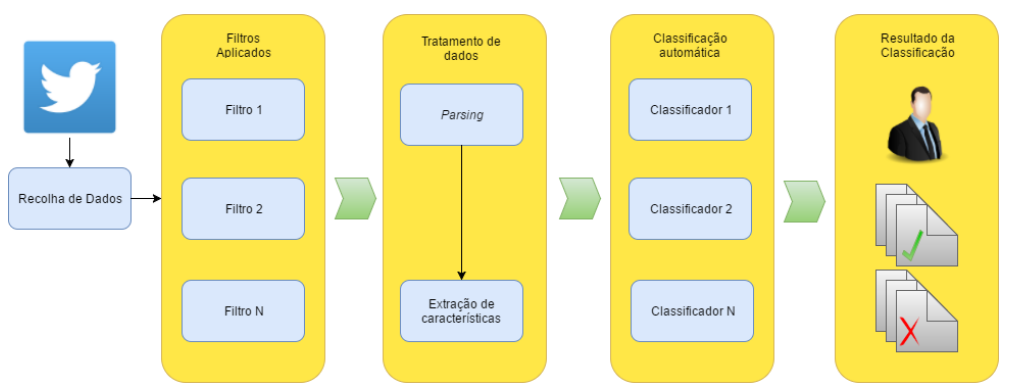
\includegraphics[width=1\textwidth]{imagens/Correia2.png}
\caption{Arquitetura do sistema proposto pelo artigo \citeonline{Correia2016} representando a forma de operação do sistema}
\label{fig:Correia2}
\end{figure}

Na fase de operação o sistema funciona de forma automática, após o treino ele consegue identificar melhor os filtros dos tweets, assim apresenta uma lista com os tweets selecionados que serão analisados por um analista posteriormente.

\citeonline{ALVESBATISTA2007} é um trabalho que estuda e apresenta dados sobre segurança em softwares e o quão difícil é de se abordar o tema colocando métricas de segurança, uma vez que nos dias atuais não é possível apresentar uma métrica quantitativa capaz de indicar o nível de segurança que o software em desenvolvimento terá \cite{ALVESBATISTA2007}. Esse trabalho tem o objetivo de comprovar essa teoria colocando a responsabilidade de segurança antes de se distribuir o software e assim sempre lançar um software fidedigno.

Com o objetivo de apresentar alguns métodos de avaliação quantitativa, apontando suas falhas, o trabalho propõe áreas de pesquisa para o estudo de métrica de seguranaça de software, para assim melhorar a avaliação. Desse modo, consegue-se a perspectiva do quão rentável é o investimento em segurança de software, a capacidade e competência de combater vulnerabilidades e como os riscos de segurança estão sendo gerenciados.

O trabalho define segurança como algo interpretativo e relativo. Quando se tem um cenário em que se coloca o nível de segurança X para um software, é relativo que a segurança do sistema tem que atende-lo no nível X. Como exemplo, um sistema de banco necessita de uma segurança alta em seu software, uma vez que um sistema de uma loja pequena de roupas de uma cidade de interior não precisa da mesma segurança. A métrica de segurança de um sistema, então, advem de sua necessidade de segurança e contexto de utilização.

\citeonline{Kroth2018} é um trabalho que busca identificar vulnerabilidades previamente definidas que estão presentes em serviços na internet, sendo esses públicos. Tem o objetivo de listar essas vulnerabilidades comuns que ataques utilizam para conseguirem acesso à informações de usuários.

O autor define que as vulnerabilidades disponíveis na rede advem de displicência por parte das organizações criadoras dos sistemas. Por parte delas o investimento em segurança não se baseia em resultado, sendo um custo sem retorno. Assim, os sistemas não têm um simples teste de invasão por uma equipe especializada, o que deixa ao público uma dúvida sobre o quão seguro o sistema é. O problema maior se encontra com o público que não conhece sobre segurança e disponibilizam seus dados em sistemas desse porte, que não tem o "selo de segurança".

O trabalho se baseia em delimitar a conexão da rede da Internet para uma rede LAN. Assim, o objetivo é encontrar vulnerabilidades previamente definidas na comunicação entre internet e LAN. Assim, o objetivo é identificar vulnerabilidade já conhecidas em sistemas em geral, contabilizando, assim, o número de sistemas que não se atualizaram, ou mesmo foram feitos, sob as medidas de segurança já definidas \cite{Kroth2018}.

Os trabahos citados têm focos diferentes nas perspectivas de segurança e objetivos diferentes. O trabalho \citeonline{Sabottke2015} e o \citeonline{Correia2016} são os que mais se aproximam com o presente trabalho, uma vez que faz também uma busca numa rede social em cima de palavras chaves e as explora para definição de vulnerabilidades em sistemas. Mas o trabalho \citeonline{ALVESBATISTA2007} se relaciona com o projeto sendo uma porta de caminho sobre o estudo de segurança do software, tendo sua base na métrica do quão um software pode ser mensurado como seguro, fazendo uma busca sobre o que seria seguro na definição de segurança de sistemas. O trabalho \citeonline{Kroth2018} também se destaco ao buscar vulnerabilidades já conhecidas pela sociedade em sistemas públicos, sendo essas vulnerabilidades já discutidas em redes sociais também. 

Existe ainda trabalhos que têm como parte do projeto a análise de dados de tweets, sendo muitos correlacionados à psicologia e estudo humano. Esses trabalho têm relação a esse pelo fato de buscar alguns filtros no Twitter. Se o presente trabalho faz uma busca por palavras chaves que retornam vulnerabilidades em sistemas, esses outros trabalhos apenas mudam a busca para conseguirem seu objetivo.

% --- Desenvolvimento --- %
% ----------------------------------------------------------
% Desenvolvimento
% ----------------------------------------------------------
\chapter[Metodologia]{Metodologia}

Neste capítulo será apresentado a metodologia feita no trabalho. Será apresentado e exemplificado o sistema criado no projeto e como foi feito as etapas para criação do mesmo. Será explicado também as tecnologias envolvidas nos sistemas.

\section{Ferramenta Desenvolvida}
Para o desenvolvimento do projeto foi desenvolvido um sistema batizado de Scanner. Esse sistema é quem faz um filtro no Twitter \cite{JackDorseyNoahGlassBizStone2006} nas suas publicações. O scanner é um sistema dividido em 3 sistemas distintos:

\begin{itemize}
\item TwitterSearch: Sistema que fornece um formulário para preenchimento dos filtros a serem utilizados na busca do Twitter.
\item Tweet: Software que faz conexão com a API de comunicação com o Twitter enviando os filtros da busca e interpretando seu retorno em uma base de dados.
\item APIConectorJson: Aplicativo que organiza a base de dados de retorno afim de organizar a informação em um banco de dados, um arquivo xml, um arquivo csv e um arquivo json.
\end{itemize}

Assim, o Scanner funciona de modo que o usuário faça sua busca no Twitter e tenha seu resultado armazenado em alguma base de dados. Então o usuário tem o total acesso dos tweets de resultado da sua busca. Esse acesso é fornecido a partir da API do GetOldTweets \cite{Pythoncommunity}. Será apresentado a seguir a especificação de cada parte do sistema infcluindo a descrição da API utilizada no trabalho.

Para esse trabalho o objetivo é levantar as vulnerabilidades discutidas na rede social Twitter. A partir dos trabalhos similares a esse, foi utilizado filtros já pré selecionados para encontrar essas vulnerabilidades. Com esses resultados, foi feito um estudo dos dados desses tweets, assim como dos usuários que os postam normalmente.

Foi criado também um sistema de busca que tem o objetivo de, a partir dos resultados do Scanner, verificar quais tweets estão realmente relacionados com alguma vulnerabilidade presente no site do NVD. Esse sistema foi batizado de FindWords. Ele será descrito nas seções posteriores.

\subsection{TwitterSearch}
Esse é um sistema cujo objetivo é acionar os demais organizando a informação dos filtros de entrada para a busca dos dados. Desenvolvido em C\#, o sistema apresenta um formulário para preenchimento dos filtros desejados e,  após preenchido o formulário pelo usuário, cria um arquivo JSON que servirá de entrada para os outros sistemas como filtro. O próprio sistema já faz a chamada dos outros aplicativos necessários.

A figura \ref{fig:TwitterSearch} apresenta a primeira parte da tela principal do sistema.

\begin{figure}[H]
\centering
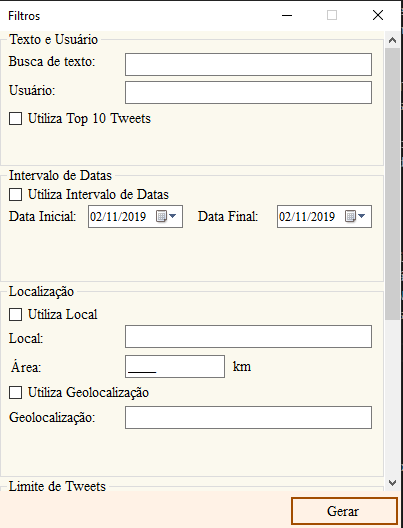
\includegraphics[width=10cm]{imagens/TwitterSearch.png}
\caption{Parte da tela principal do sistema}
\label{fig:TwitterSearch}
\end{figure}

Essa tela apresenta os dados do formulário referente a:

\begin{itemize}
\item Texto e Usuário:

\begin{itemize}
\item Busca de Texto: Essa busca irá filtrar no Twitter publicações que, em seu conteúdo, tenham a palabra digitada. Vale ressaltar que essa palavta será comparada de forma limpa e completa, ou seja, o texto para ser considerado igual deve ter a mesma palavra em seu conteúdo, não apenas parte dela.
\item Usuário: Irá pesquisar na rede social publicações do usuário digitado. Esse usuário é o nome que o mesmo utiliza na rede.
\item Utiliza Top 10 Tweets: Essa opção selecionará os Top 10 tweets do usuário digitado na opção anterior. Esse top 10 significa os 10 tweets mais importante daquele usuário, ou seja, os que faram mais retweetados e curtidos.
\item Usuário: Irá pesquisar na rede social publicações do usuário digitado. Esse usuário é o nome que o mesmo utiliza na rede.
\end{itemize}

\item Intervalo de Datas

\begin{itemize}
\item Utiliza Intervalo de datas: Essa opção ativa o intervalo de datas. Se selecionada, o sistema irá filtrar a data da pubicação do tweet no intervalo das datas selecionadas nos combos.
\item Data Inicial: Data inicial a se considerar os tweets do filtro. A data inicial é incluída no filtro também, ou seja, tweets publicados no dia selecionado também serão retornados.
\item Data Final: Data final a se considerar os tweets do filtro. A data final é incluída no filtro também, ou seja, tweets publicados no dia selecionado também serão retornados.
\end{itemize}

\item Localização

\begin{itemize}
\item Utiliza Local: Essa opção atia o filtro de localização onde o tweet foi publicado. Essa opção não considera a localização do usuário que postou o tweet, mas sim a localização que estava no momento que que foi publicado.
\item Local: Esse filtro pode considerar cidade, estado, país ou mesmo região. Um exemplo de utilização seria: Berlin, Germany.
\item Área: Perímetro a se considerar a partir do local selecionado. Uma opção de entrada seria 50km, então utilizando a opção anterior, de Berlin, esse filtro contataria até 50km em volta dessa cidade. 

\item Utiliza Geolocalização: Essa opção permite que o usuário utiliza geolocalização para filtrar os tweets. assim como o Local, a geolocalização irá identificar a partir do local em que o tweet foi publicado.
\item Geolocalização: Entrada de latitude e longitude. Um de entrada exemplo seria: 55.75, 37.61. A Área, já mencionada, também funciona se preenchida assim como a geolocalização.
\end{itemize}

\end{itemize}

Essa é a primeira tela do sistema. Esses filtros colocados são os principais e comumente mais utilizados. O trabalho \citeonline{Sabottke2015} utiliza filtro de texto e data para obtenção dos resultados. Em sua pesquisa, os dados têm por base o ano de 2015 filtrando a palabra CVE, que é a sigla utilizada para filtro de vulnerabilidades \cite{CVE1985}.

A figura \ref{fig:TwitterSearch2} apresenta a segunda parte da tela principal do sistema. Como o número de filtros é grande, o sistema acaba tendo uma barra de rolagem que disponibiliza o restante dos filtros.

\begin{figure}[H]
\centering
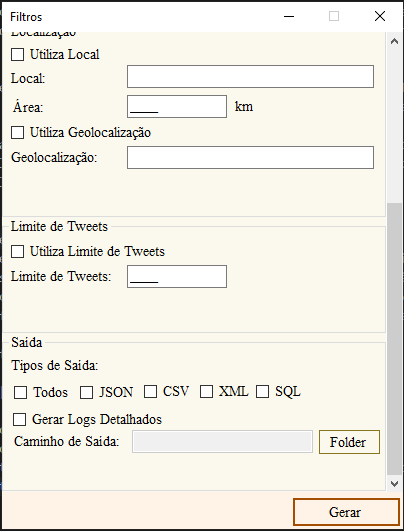
\includegraphics[width=10cm]{imagens/TwitterSearch2.png}
\caption{Segunda Parte da tela principal do sistema}
\label{fig:TwitterSearch2}
\end{figure}

A sequnência da tela apresenta os dados do formulário referente a:

\begin{itemize}

\item Limite de Tweets

\begin{itemize}
\item Utiliza Limite de Tweets: Essa opção valida se vai limitar o número de tweets no retorno da bucsa.
\item Limite: Número de Tweets máximo de retorno da consulta
\end{itemize}

\item Saída

\begin{itemize}
\item Tipos de Saída: Essa opção seleciona qual o tipo de saída do programa: JSON, CSV, XML, SQL.
\item Gerar Logs Detalhados: Essa opção faz com que os sistemas gerem um log detalhado sobre suas atividades.
\item Caminho de Saída: Essa opção permite que o usuário selecione onde os arquivos de saída devem ser copiados.
\end{itemize}

\end{itemize}

Esse sistema é a primeira parte do trabalho, cujo objetivo é apenas apresentar o formulário e, a partir do preenchimento dele, gerar um arquivo JSON de configuração de filtro de entrada para os outros arquivos.
 
\subsection{Tweet}

Esse sistema foi desenvolvido em Python e tem o objetivo de fazer a conexão com a API do GetOldTweets \cite{Pythoncommunity}. Para sua execução, ele precisa de um arquivo de entrada que contenha as informações dos filtros que será colocado na busca dos tweets. A imagem \ref{fig:entradaTweet} mostra um exemplo de um arquivo de entrada desse sistema.

\begin{figure}[H]
\centering
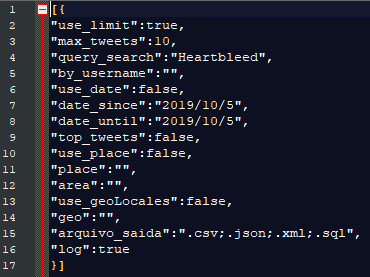
\includegraphics[width=8cm]{imagens/entradaTweet.png}
\caption{Exemplo de entrada do programa Tweet}
\label{fig:entradaTweet}
\end{figure}

Esses filtros são os enviados ao GetOldTweets\cite{Pythoncommunity} para obter o retorno. Desse retorno, para cada tweet x de resultado, é buscado o TOP 10 dos tweets referente àquele usuário que publicou o tweet x.

O sistema conta ainda com a opção de log, na figura \ref{fig:entradaTweet} apresentado na tag "log". Essa opção faz com que cada passou do sistema seja relatado em um arquivo de log no caminho: raiz da aplicação/log/"data do log". Essa opção é importante, pois nem sempre a API está funcionando corretamente, o que faz com que o sistema apresente lentidão em sua execução. 

Ademais, o sistema faz uma interação com o usuário afim de apresentar em qual parte da análise está sendo efetuada, conforme imagem \ref{fig:TweetExecucao}.

\begin{figure}[H]
\centering
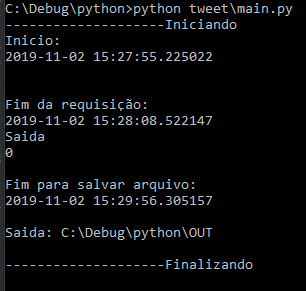
\includegraphics[width=8cm]{imagens/TweetExecucao.png}
\caption{Exemplo de execução do sistema Tweet}
\label{fig:TweetExecucao}
\end{figure}

O sistema apresenta a data e hora de início da execução. Após isso ele começa a realizar a requisição da API, quando finalizado apresenta a data e hora de finalização requisição. Após isso o Tweet chama a aplicação APIConectorJson, que faz o tratamento dos dados, quando finalizado apresenta data e hora da finalização do taratamento dos dados. Apresenta ainda a saída da requisição: 0 para sucesso e qualquer outro para código de erro do sistema operacional. No final apresenta o caminho onde os arquivos foram salvos.

O sistema funciona então em duas fases: (1) seleciona os filtros no arquivo de entrada e faz a requisição com a API gerando um arquivo de saída X e (2) seleciona esse arquivo de saída e chama o aplicativo APIConectorJson passando o arquivo X como entrada e passando quais são os tipos de saída desejados. 

\subsection{API GetOldTweets}

A API do GetOldTweets é uma biblioteca desenvolvida em python que tem o objetivo de fazer uma busca no Twitter apartir dos filtros possíveis, que serão descritos posteriormente. Seu funcionamento se baseia na leitura de um brownser que acessa a rede social, então o resultado é obtido a partir dessa busca. Logo, o resultado sempre fica ordenado de forma cronológica, ou seja, pela data da publicação.

Essa API possui vários recursos para ser utilizado, não se limitando apenas à uma bilioteca. É possível acessa-la através de linha de comando pelo CMD passando os parâmetros de busca, assim como é possível chama-la a partir de um programa externo, seja em python ou não. Cada uma das formas de chama-la gera um resultado diferente: se chamado por linha de comando é gerado um arquivo CSV com as informações, já chamando a partir de um programa externo a bilioteca retorna um arquivo JSON com os tweets. A estrutura dos objetos de retorno é dada com os seguintes atributos:

\begin{itemize}
\item id (string); Código referente ao tweet
\item permalink (string); Link da publicação
\item username (string); Nome do usuário que fez a publicação
\item text (string); Texto do tweet
\item date (datetime); Data da publicação
\item retweets (integer); Número de vezes que o tweet foi retweetado
\item favorites (integer); Número de vezes que o tweet foi favoritado
\item mentions (string); Lista as menções da publicação
\item hashtags (string); Apresneta as hashtags da publicação
\item geo (string); Localização onde o tweet foi publicado
\end{itemize}

Para o presente trabalho foi escolhido utilizar a API como uma biblioteca de um sistema externo, então é conectado na API e retornado o arquivo JSON com os dados da busca. 

A biblioteca funciona em duas partes: listar os filtros para a busca (classe TwitterCriteria) e realizar a busca propriamente dita (TweetManager). A classe de organização das buscas possui os seguintes métodos que possibilitam a realização dos filtros:

\begin{itemize}
\item setUsername (str or iterable): Nome do usuário para a busca
\item setSince (str. "yyyy-mm-dd"): Data de início da busca. Se não for dado um valor não há limite de busca. Se setado um valor esse é incluído no resultado, ou seja, se colocado a data 2015-01-01 no resultado haverá tweets dessa data.
\item setUntil (str. "yyyy-mm-dd"): Data final da busca. Se não colocado a data final será o dia em que a busca foi realizada, com resultados incluindo esse dia. Se setado o dia colocado não é considerado no resultado, ou seja, se colocado 2015-12-31 não haverá tweets dessa data.
\item setQuerySearch (str): Texto para verificação no Twitter. Esse texto será buscado na rede como um todo e deve haver um "match" completo da palavra para o tweets ser considerado resultado da busca. Ou seja, se filtrado a palavra "CVE", como será feito por esse trabalho, será retornado todos os tweets da rede que tenham essa palavra. A busca não é case sensitive, ou seja, não importa texto em maiúsculo e minúsculo.
\item setTopTweets (bool): Se setado como "true" é retornado apenas os Top tweets. Esse conceito de Top tweet se baseio no número de curtida e número de seguidores do usuário que publicou o tweet.
\item setNear(str): Uma referência de área localização onde o tweet foi publicado. 
\item setWithin (str): Filtra a busca por uma área de localização a partir da opção colocada no setNear.
\item setMaxTweets (int): O número máximo de tweets a ser suportado na busca dos dados. Se não setado ou se o valor for menor que 1 será retornado a busca total dos tweets, sem limite.
\end{itemize}

A biblioteca possui ainda algumas limitações baseada nas condições em que a busca é efetuada. Basicamente, se a rede for oscilante no momento de leitura e requisição dos dados é possível que o retorno não seja composto por todos os tweets da busca, uma vez que a API faz uma busca na rede social lendo um brownser, ou seja, se não carregar os dados no navegador a biblioteca não terá nada para ler, ou se carregar apenas parte irá retornar apenas esse trecho de resultado. Para facilitar a busca de ocorrência desse problema basta conferir no resultado a data do último tweet retornado, se a data for uma não reconhecida, ou seja, não for a desejada, houve erro na busca. Esse erro também pode ocorrer devido ao estouro da memória principal, pois a API faz a busca utilizando dessa memória para armazenamento dos dados para apenas depois montar o arquivo de saída.

Para o presente trabalho foi enfrentado ambos os problemas. Como será citado nos resultado, a busca foi feita para o ano de 2019, mas comparando aos resultados dos anos anteriores (2018, 2017, 2016 e 2015), e para a busca de todo esse período foi encontrado certa dificuldade por limitação de rede e de memória.

\subsection{APIConectorJson}

Essa parte do sistema funciona com o propósito de organizar as informações obtidas da API GetOldTweets \cite{Pythoncommunity}. Ele recebe de entrada um arquivo JSON com os dados da requisição e recebe também quais são as saídas esperadas conforme citado na seção anterior. Desse arquivo é retirado todos os objetos e para cada um dos tipos de saída é feito um tratamento diferente. Além disso, todo o processo também pode ser logado caso haja alguma espécie de erro. Esse log é o mesmo do sistema Tweet.

Os tipos de saída são configurados da seguinte forma:

\begin{itemize}
\item JSON: Arquivo com estrutura pré estabelecida, é um modelo para armazenamento e transmissão de informações no formato texto e que é bastante utilizado por aplicações Web que trabalham com a tecnologia AJAX. É um objeto JavaScript. A própria API do GetOldTweets \cite{Pythoncommunity} retorna o arquivo JSON com o resultado, então o sistema só copia o arquivo para a pasta de saída.  
\item CSV: Arquivo com a estrutura de informações separados por vírgulas. Comunmente utilizado para apresentação de informações em planílhas e cópias de dados entre bases de informações, como banco de dados. Esse tipo de armazenamento agrupa as informações de texto em planilhas. O sistema o utiliza colocando os tipos na primeira linha do arquivo e as informações nas demais.
\item XML: é um tipo de armazenamento que utiliza a linguagem de marcação recomendado pela W3C. É utilizado para representação de dados de forma estruturada mantendo as informações de acordo com suas especificidades. Utiliza de tags para caracterizar uma informação. O sistema utiliza as tags colocando os tipos dos dados nelas e a informação no espaço restante.
\item SQL: é um armazenamento em banco de dados comum, tabelado. A informação é colocada em uma tabela onde a coluna é o tipo de informação e as linhas são as tuplas de informações. O sistema utiliza esse tipo colocando os tipos dos tweets como as colunas da tabela RETORNO e as linhas são os tweets que estavam no arquivo JSON de entrada.
\end{itemize}

O sistema então tem como objetivo organizar os dados do arquivo de entrada nos aruqivos de saída. Ele trabalha apenas com essa função, possibilitando que qualquer arquivo de entrada JSON tenha sua saída nos tipos permitidos de dados: JSON, CSV, XML e SQL. 

\subsection{Scanner}

O conjunto dos sistemas anteriormente citados dá origem ao sistema Scanner. Esse possui a interface do TwitterSearch, o que possibilita preenchimento do formulário disponibilizando um arquivo JSON de configuração de filtragem e que chama o "cérebro" do programa: o Tweet. Este processa o arquivo de entrada com os filtros requisitando a API GetOldTweets \cite{Pythoncommunity} com esses dados, obtendo os tweets de retorno que satisfazem a busca, criando um novo arquivo json de saída contendo uma lista com os objetos dos tweets retornados pela API. Assim chama o APIConectorJson para organização dos dados passando o JSON com os objetos dos tweets e passando os tipos de saída selecionado no TwitterSearch, depois de finalizado o próprio Tweet copia as saídas para o caminho selecionado pelo usuário.

Um exemplo de funcionalidade segue na figura \ref{fig:entrada1} que apresenta as seguintes entradas.

\begin{figure}[H]
\centering
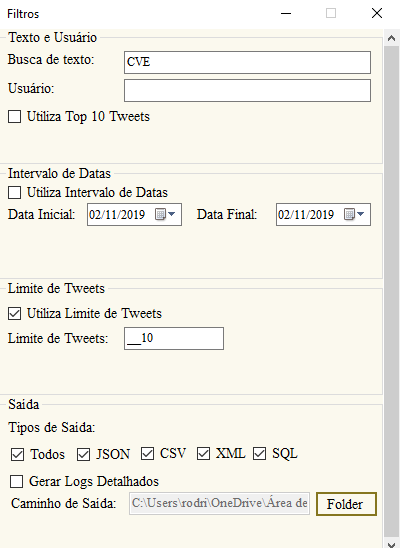
\includegraphics[width=10cm]{imagens/entrada1.png}
\caption{Entrada de exemplo (imagem editada com o propósito de listar apenas os filtros utilizados)}
\label{fig:entrada1}
\end{figure}

Com essas estradas, o sistema chama as outras aplicações e obtem as saídas nos arquivo em JSON, CSV, XML e SQL. Todos esses arquivos possuem os dados de retorno do Twitter com a busca feita. Tomando como exemplo um desses tweets do retorno da busca, o de ID 1190312935895158789 do usuário Tribe\_Secure, ele é listadas nas figuras \ref{fig:saidaJson}, \ref{fig:saidaCSV}, \ref{fig:saidaXML} e \ref{fig:saidaSQL}.

\begin{figure}[H]
\centering
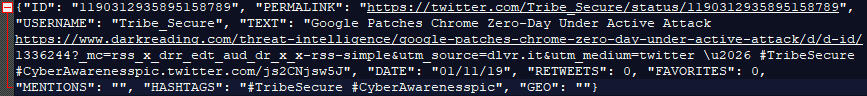
\includegraphics[width=1\textwidth]{imagens/saidaJson.png}
\caption{Exemplo do tweet em saída JSON (o texto foi alinhado para uma melhor visualização)}
\label{fig:saidaJson}
\end{figure}

\begin{figure}[H]
\centering
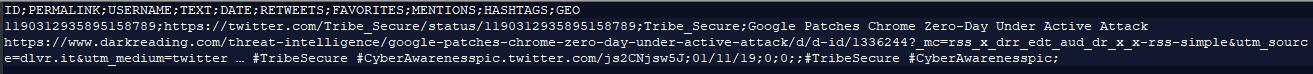
\includegraphics[width=1\textwidth]{imagens/saidaCSV.png}
\caption{Exemplo do tweet em saída CSV}
\label{fig:saidaCSV}
\end{figure}

\begin{figure}[H]
\centering
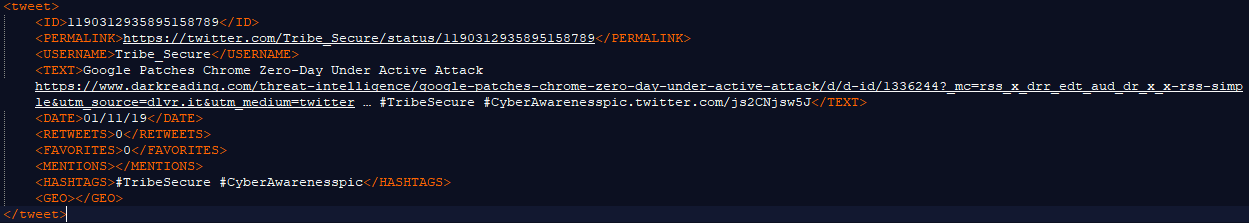
\includegraphics[width=1\textwidth]{imagens/saidaXML.png}
\caption{Exemplo do tweet em saída XML}
\label{fig:saidaXML}
\end{figure}

\begin{figure}[H]
\centering
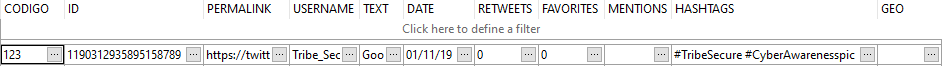
\includegraphics[width=1\textwidth]{imagens/saidaSQL.png}
\caption{Exemplo do tweet em saída SQL}
\label{fig:saidaSQL}
\end{figure}

O exemplo de entrada ainda será utilizado nesse trabalho, filtrando ainda por data. Como o retorno monta uma base de dados consideravelmente grande, ele já mostra que o volume de dados de quando não se coloca limite de número de tweets pode crescer ainda mais. A fim de teste, foi colocado uma busca com um número ilimitado de tweets e sem fechar nenhuma data, como resultado passaram-se mais de 24 horas e o programa ainda não tinha finalizado suas solicitações.

Esse é o sistema no qual o trabalho se baseia. É com ele que a análise sobre as quantidade de vulnerabilidades discutidas no Twitter será possível, assim como a frenquência da mesma nos últimos anos. Esse é um programa genérico que possibilita buscas em toda a rede, logo será nossos filtros que farão com que a busca seja orientada aos objetivos do trabalho.

\subsection{FindWords}

Esse sistema tem como objetivo buscar uma palavra (ou parte dela) em arquivos de diretórios distintos. Dado um diretório A e a palavra "CVE", o programa irá listar como resultado todos os arquivos da pasta e subpasta do diretório A que conténham essa palavra e em qual linha do arquivo a mesma está. 

O objetivo desse programa é buscar para cada resultado do Scanner o código CVE publicado nas listas presente no site NVD. A partir desse resultado é possível verificar quais vulnerabilidades estão sendo discutidas e realmente existem no cite do CVE e do NVD.

O programa possibilita ler todos os possíveis arquivos de saída do Scanner (XML, JSON, CSV e SQL) e, a partir desses arquivos, ler o código descrito na publicação no Twitter e buscar esse código nas bases de conhecimento do NVD.

O resultado dessa busca é um arquivo txt de saída que lista o código CVE encontrado no tweet e o diretório do arquivo e linha do arquivo em que o mesmo código foi encontrado.

Há ainda a possibilidade de, ao invés de procurar nos arquivos do diretório selecionado, utilizar um banco de dados para a busca da palavras.

\section{Coleta de dados}

O Scanner faz uma busca no Twitter a partir da API GetOldTweets \cite{Pythoncommunity} passando os parâmetros de filtro. Essa é a coleta de dados que o sistema faz da rede social. 

Para trabalhar com os dados, eles são organizados em outros arquivos que possibilitam a visualização melhor dos dados, assim o trabalho de análise fica mais simples.

O site do NVD, como já foi citado, apresenta uma lista de opção para download das vulnerabilidades. O site organiza essas informações colocando-as em um arquivo ZIP para cada ano \cite{NISTDownload}. Assim, é possível baixar essas informações e utilizar delas para analisar os dados de retorno. O site do CVE também fornece a opção de baixar o um arquivo XML com os mesmos dados, mas o arquivo não é em formato ZIP e acaba sendo um pouco maior para download \cite{TheMITRECorporation2018}.

A coleta de dados então é feita a partir de duas bases para a análise desse trabalho: Twiiter, através da API do GetOldTweets \cite{Pythoncommunity}; e o NVD, que processa seus dados a partir da base do CVE.

Tomando como exemplo a figura \ref{fig:exemploVulnerabilidade}, tem-se a vulnerabilidade de código CVE-2019-2110. A figura \ref{fig:exemploVulnerabilidadeCVE} apresenta suas informações no site do CVE.

\begin{figure}[H]
\centering
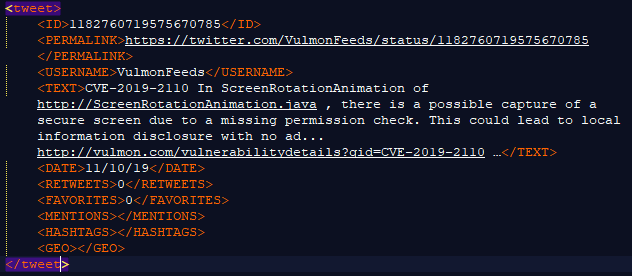
\includegraphics[width=1\textwidth]{imagens/exemploVulnerabilidade.png}
\caption{Exemplo de publicação de uma vulnerabilidade no Twitter em formato xml}
\label{fig:exemploVulnerabilidade}
\end{figure}

\begin{figure}[H]
\centering
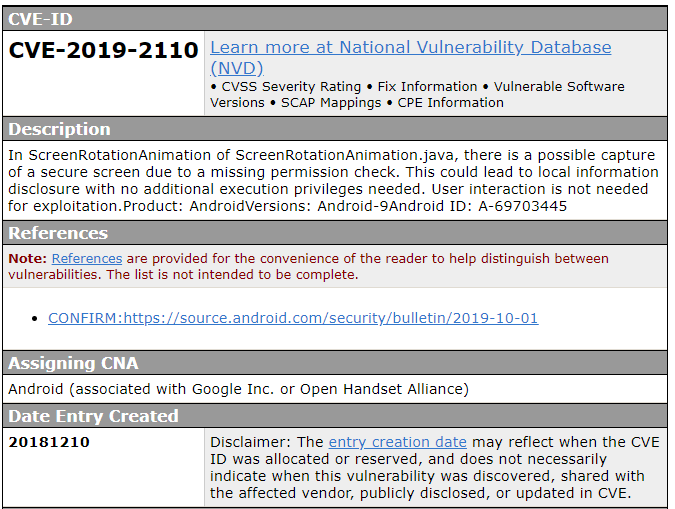
\includegraphics[width=1\textwidth]{imagens/exemploVulnerabilidadeCVE.png}
\caption{Descrição da vulnerabilidade CVE-2019-2110 no site do CVE \cite{CVE1985}}
\label{fig:exemploVulnerabilidadeCVE}
\end{figure}

O arquivo disponibilizado no site do NVD referente ao ano de 2019 descreve a vulnerabilidade, como apresentado na figura \ref{fig:descricaoVulnerabilidadeNVD}. Assim como o arquivo XML baixado no site do CVE, apresentado na figura \ref{fig:descricaoVulnerabilidadeCVE}.

\begin{figure}[H]
\centering
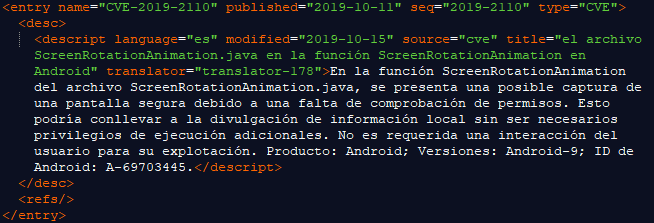
\includegraphics[width=1\textwidth]{imagens/descricaoVulnerabilidadeNVD.png}
\caption{Descrição da vulnerabilidade CVE-2019-2110 no arquivo disponibilizado no NVD}
\label{fig:descricaoVulnerabilidadeNVD}
\end{figure}

\begin{figure}[H]
\centering
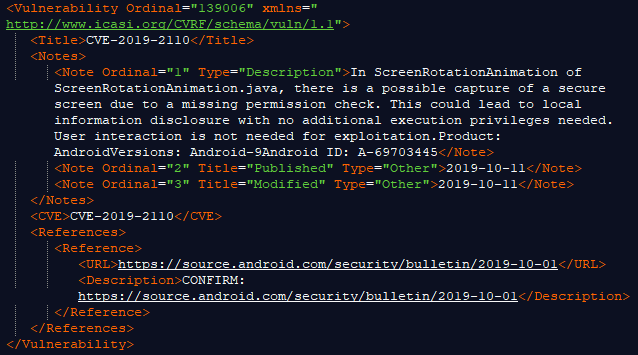
\includegraphics[width=1\textwidth]{imagens/descricaoVulnerabilidadeCVE.png}
\caption{Descrição da vulnerabilidade CVE-2019-2110 no arquivo disponibilizado no CVE}
\label{fig:descricaoVulnerabilidadeCVE}
\end{figure}

A coleta dos dados então não se restringe apenas ao Twitter, mesmo que o objetivo seja a verificação de discussão sobre vulnerabilidades na rede social. A coleta é feita nos sites que tratam de vulnerabilidades para a identificação correta do que é ou não vulnerabilidade. Parte da análise está em filtrar na rede social, a outra está na identificação dessas vulnerabilidades.

Para o presente trabalho os filtros foram feito para esse ano (o objetivo é identificar como a discussão está hoje!). Logo, tanto no site do NVD quanto no CVE foi baixado os arquivos referente ao ano de 2019 e os mesmos serão utilizados em conjunto com o filtro feito de publicações do ano de 2019 por parte do Scanner.

Então o Scanner é o responsável por buscar esses dados do Twitter e o FindWords será o responsável por relacionar os dados recolhidos da rede social com os dados presentes nos sites do CVE e do NVD.

No próximo capítulo será listado os resultados dessas buscas comparando outros anos. O número de vulnerabilidades tem crescido exponencialmente, isso é fato, o CVE prova isso a partir dos tamanhos dos arquivos de cada ano. Esse aumento também é experado no número de pessoas discutindo o tema no Twitter. 



% --- Conclusão --- %
% ----------------------------------------------------------
% Resultados
% ----------------------------------------------------------
\chapter[Resultados]{Resultados}

Esse capítulo apresentará os resultados do presente trabalho apresentando gráficos, tabelas e imagens que mostram como foi a resposta obtida do programa criado (Scanner). O capítulo é separado primeiramente pela apresentação dos dados concretizados e como se chegou a eles, posteriormente será apresentado uma comparação com os outros trabalhos. O objetivo é explicar os seguintes pontos:

\begin{itemize}
\item A discussão sobre vulnerabilidades de segurança em redes sociais está aumentando ao longo do tempo assim como a descoberta de nuvas vulnerabilidades?
\item Quais são os tipos de vulnerabilidades com maior insidência de discussão na rede?
\item Qual a razão entre vulnerabilidades de segurança discutidas em redes sociais e vulnerabilidades descobertas?
\item A partir dos resultados das vulnerabilidades encontradas, quais já possuem um exploit?
\end{itemize}

A partir dessas perguntas é possível entender se o tema de vulnerabilidade está ganhando maior interesse por parte de organizações e pela sociedade. Se um dos pilares da humanidade está sendo a tecnologia é preciso que a segurança esteja atrelada a isso, então é necessário que exista pesquisas para o desenvolvimento dessa área.

\section{Análise dos dados}

Para chegar ao objetivo do trabalho foi feito um levantamento da quantidade de vulnerabilidades que foram discutidas no ano de 2019 na rede social do Twitter. Utilizando a ferramenta do Scanner foi feito o filtro nesse período e, a partir dos resultados, foi vinculado à lista do site do CVE para identificação da existência da vulnerabilidade discutida atravé do FindWords. 

Como base de comparação, foi feito também o levantamento para os anos de 2015, 2016, 2017, 2018 e 2019. O filtro utilizado foi o mesmo, palavra 'CVE' para busca, diferenciando-se apenas no intervalo de datas.

%A tabela \ref{tab:tabela1} apresenta a relação entre ano x número de tweets com a palavra chave CVE x número de CVE existentes também no site do NVD.

%\begin{table}[H]
%\centering
%\caption{Índices Sazonais de Descoberta de Vulnerabilidades - Web}
%\label{tab:tabela1}
%\includegraphics[width=.7\textwidth]{imagens/tabela1_Vulnerabilidades.png}
%\end{table}

% --- Conclusão --- %
% ----------------------------------------------------------
% Conclusão
% ----------------------------------------------------------
\chapter[Conclusão]{Conclusão}

% ----------------------------------------------------------
% ELEMENTOS PÓS-TEXTUAIS
% ----------------------------------------------------------
\postextual

% --- Referências bibliográficas --- %
\bibliography{bibliografia}

% --- Apêndices --- %
% só mantenha se for pertinente.
%\begin{apendicesenv}
%\partapendices % Imprime uma página indicando o início dos apêndices

% --- Apendice 1--- %
%% ----------------------------------------------------------
% Apendice 1
% ----------------------------------------------------------
\chapter{Coisas que fiz e que achei interessante mas não tanto para entrar no corpo do texto}

\lipsum[50]

%\end{apendicesenv}

% --- Anexos --- %
% so mantenha se pertinente.
%\begin{anexosenv}
%\partanexos % Imprime uma página indicando o início dos anexos

% --- Anexo 1 --- %
%% ----------------------------------------------------------
% Anexo 1
% ----------------------------------------------------------
\chapter{Coisas que eu não fiz mas que achei interessante o suficiente para colocar aqui}


\lipsum[31]

%\end{anexosenv}


% ------------------------------------------------------------------------
% FIM DO DOCUMENTO
% ------------------------------------------------------------------------
\printindex
\end{document}